\section{Measurement and Density/Relative Density}

Human progress is due, in large part, to an ability to measure and hence collect data with
greater and greater precision. Young students should learn, generally, about how to obtain data
by carrying out simple experiments. They should be introduced to the basic measurements of
mass, distance and time. They should be trained in recording and in graphical analysis of
data.

\begin{multicols}{2}

\section*{Collection of Data}


\subsection{Data on Weighing}

\begin{center}
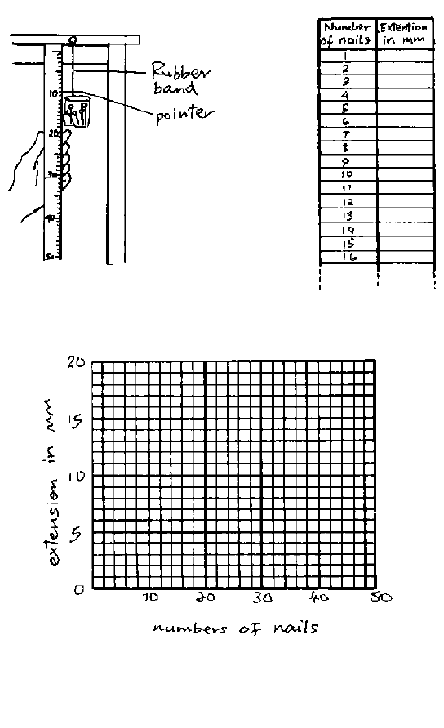
\includegraphics[width=0.5\textwidth]{./img/source/meas-mass.png}
\end{center}

Fix a rubber band at one end to a table or retort stand. At the other end, attach a paper clip to act as a pointer and a small bag or scale pan. Fill the bag or scale pan with successive numbers of nails. Have students measure the extension of the rubber band each time they add more nails. Record the readings and use the data to draw a graph as shown in the figure.

\vfill
\columnbreak

\subsection{Data on Distance}

\begin{center}
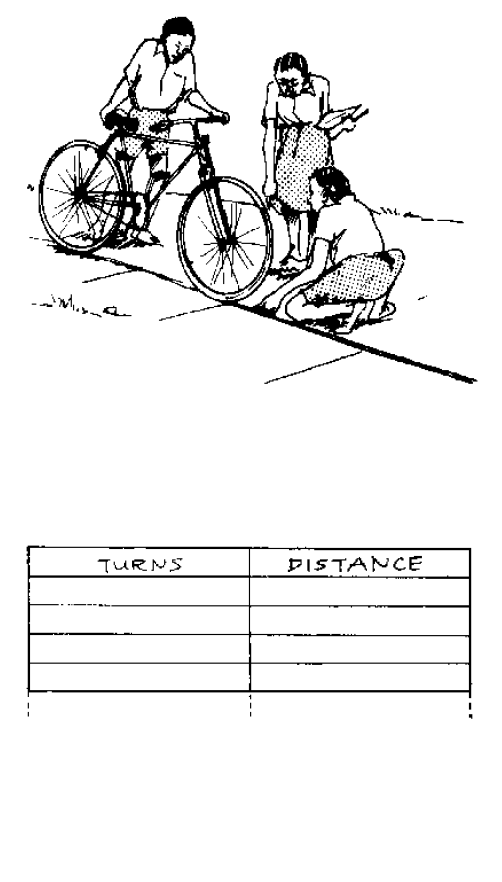
\includegraphics[width=0.5\textwidth]{./img/source/meas-distance.png}
\end{center}

Make a mark on the tyre of a bicycle at the point where it touches the ground. Turn the tyre by moving the bicycle forward and record the length of one turn. Repeat the experiment several times for various numbers of turns, each time recording the horizontal distance covered. Draw a graph to show the data.

\vfill
\columnbreak

\subsection{Data on Time}

\begin{center}
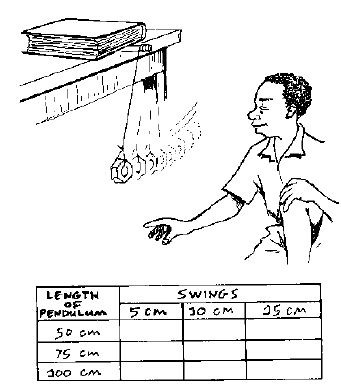
\includegraphics[width=0.5\textwidth]{./img/source/meas-time.png}
\end{center}

Fix a string just off the edge of a table and hang a small weight (e.g. a nut or nail) at a distance of 50 cm. This is a simple pendulum. Pull the pendulum to one side so that its horizontal displacement is 5 cm. Count the number of oscillations (back and forth) made in one minute. Repeat by increasing the horizontal displacement to 10 cm and 15 cm. Then try varying the length of the string. How long must the pendulum be to oscillate 60 times in one minute?

\vfill
\columnbreak

\subsection{Data on Velocity}

\begin{center}
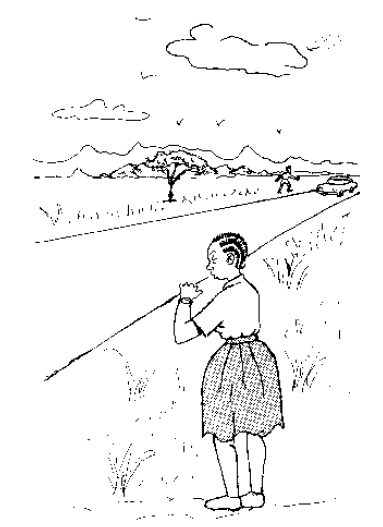
\includegraphics[width=0.5\textwidth]{./img/source/meas-velocity.png}
\end{center}

Mark a distance of 100 metres along a nearby road or playground. Note the time taken for a
car, a bicycle or a sprinter to cover the distance as follows. One pupil waves down his hand
as either the car, bicycle or sprinter crosses the 0 metres mark. Another pupil with a watch,
starts timing at the same time. A third pupil at the 100 metre mark waves down his hand as
the moving object crosses the 100 metre mark and at this instant the timekeeper stops his
watch.

\vfill
\columnbreak

%\subsection{Mass vs. Weight}

%==================================================================================================%

\section*{Measuring Instruments}


\subsection{Construction of a Metre Rule}
\label{sub:metrerule}

\begin{description*}
%\item[Subtopic:]{Concept of Measurement}
\item[Materials:]{Wooden board, pen\slash pencil, a handsaw, ruler or tape measure}
%\item[Setup:]{}
\item[Procedure:]{Use the handsaw to cut a piece of wood 100 cm $\times$ 3.5 cm $\times$ 0.5 cm. Use a ruler or tape measure to mark a scale in cm on the wood.}
%\item[Hazards:]{}
%\item[Questions:]{}
%\item[Observations:]{}
%\item[Theory:]{}
\item[Applications:]{Students can record data on their height, dimensions of the classroom, etc.}
\item[Notes:]{Instead of a wooden block, string can be used by making knots at different intervals.}
\end{description*}

\subsection[Construction of a Beam Balance]{Construction of a Beam \hfill \\ Balance}
\label{sub:beambalance}

\begin{center}
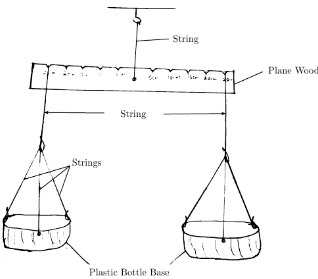
\includegraphics[width=0.5\textwidth]{./img/beam-balance.png}
%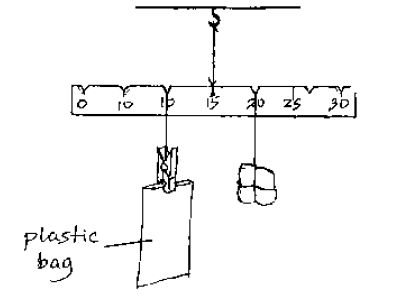
\includegraphics[width=0.4\textwidth]{./img/source/simple-balances.png}
\end{center}

\begin{description*}
%\item[Subtopic:]{Concept of Measurement}
\item[Materials:]{Ruler or wooden bar 30 cm $\times$ 2 cm, nails, razor/knife, string/wire, pen, 2 \nameref{sub:scalepans}}
%\item[Setup:]{}
\item[Procedure:]{Find the balancing point of the ruler and mark it with a pen. Use a heated nail to make a hole through this point. Make notches at 5 cm intervals on either side of the center hole using a razor/knife to suspend scale pans. Suspend the balance with a string/wire.}
%\item[Hazards:]{}
%\item[Questions:]{}
%\item[Observations:]{}
%\item[Theory:]{}
%\item[Applications:]{Principle of Moments}
\item[Notes:]{Use locally available \nameref{sec:masses} to find the mass of everyday objects, e.g. notebooks, pens, rulers.}
\end{description*}

\columnbreak

\subsection{Scale Pans}
\label{sub:scalepans}

\begin{center}
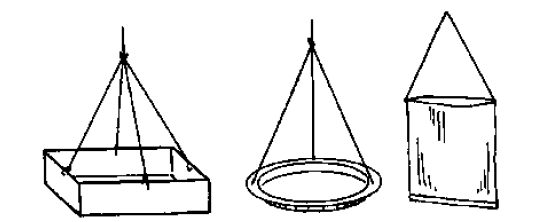
\includegraphics[width=0.4\textwidth]{./img/source/scale-pans.png}
\end{center}

\begin{description*}
%\item[Subtopic:]{Concept of Measurement}
\item[Materials:]{Match boxes, large plastic bottles, tin can lids, small plastic bags, knife, string}
%\item[Setup:]{}
\item[Procedure:]{Use a knife to poke 3~-~4 holes in the sides of one of the above materials. If using plastic bottles, cut them about 3~-~4~cm from the bottom. Cut equal lengths of string and tie them through the holes in the scale pan. Join the strings together at the upper end. }
%\item[Hazards:]{}
%\item[Questions:]{}
%\item[Observations:]{}
%\item[Theory:]{}
%\item[Applications:]{}
%\item[Notes:]{}
\end{description*}

\subsection{Construction of a Measuring Cylinder}
\label{sub:meascyl}

%\begin{center}
%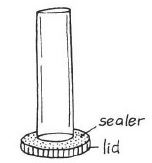
\includegraphics[width=0.2\textwidth]{./img/vso/meas-cyl.jpg}
%\end{center}

\begin{description*}
%\item[Subtopic:]{Concept of Measurement}
\item[Materials:]{Plastic bottles of different sizes, syringes (10 mL - 50 mL), marker pen, ruler, bucket of water}
%\item[Setup:]{}
\item[Procedure:]{Using the syringe, transfer a known volume of water from the bucket to the empty bottle. Use the marker pen to mark the level of water on the bottle. Repeat for a range of volumes, using a ruler to complete the scale.}
%\item[Hazards:]{}
%\item[Questions:]{}
%\item[Observations:]{}
%\item[Theory:]{}
%\item[Applications:]{}
%\item[Notes:]{}
\end{description*}

\subsection{Construction of a Eureka Can}
\label{sub:eurekacan}

\begin{center}
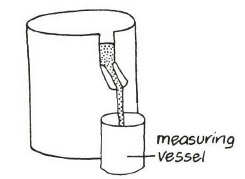
\includegraphics[width=0.3\textwidth]{./img/vso/overflow-can.jpg}
\end{center}

\begin{description*}
%\item[Subtopic:]{Determining the Volume of Irregular Objects}
\item[Materials:]{Plastic bottle, knife}
%\item[Setup:]{}
\item[Procedure:]{Cut a plastic bottle about 10~cm from the bottom. Cut 2 slits at the top of the bottle and bend the strip forward to form a spout.}
%\item[Hazards:]{}
%\item[Questions:]{}
%\item[Observations:]{}
%\item[Theory:]{}
\item[Applications:]{Measuring the volume of irregular objects, Archimedes' Principle}
\item[Notes:]{Alternatively, use a bottle or tin can and poke a hole near the top using a heated nail. Attach a straw/hollow pen tube/tube of aluminum foil, using super glue to ensure an air-tight seal.}
\end{description*}

\columnbreak

\subsection{Errors in Measurement}
\label{sub:meas-errors}

\begin{description*}
%\item[Subtopic:]{}
\item[Materials:]{Metre rules, stopwatches}
%\item[Setup:]{}
\item[Procedure:]{(a) Draw a line on the board or floor. Have several students measure the length and secretly record their results. Collect the results and record them on the board, noting any differences.\\(b) Distribute stopwatches to several students. Clap twice and have students measure the time betweeen claps and secretly record their results. Collect the results and record them on the board, observing any differences.}
%\item[Hazards:]{}
\item[Questions:]{What is the best result to use for each of the collected measurements?}
%\item[Observations:]{}
\item[Theory:]{Measurements vary from person to person. Every measurement comes with some level of error, and so it is important to take care when measuring to increase accuracy. The best result to use is the average of all the measurements.}
%\item[Applications:]{}
%\item[Notes:]{}
\end{description*}

%==================================================================================================%

\section*{Density/Relative Density}

%Density can be found by taking the ratio of a body's mass to its volume. Common units of density are g/mL and kg/L. $$ \mathrm{Density} = \mathrm{mass} \div \mathrm{Volume} $$$$ \rho = \cfrac{m}{V} $$
%Relative density (R.D.) can be used to compare the density of a given material to that of water.  Water is the standard with a density of 1.0 g/cm$^3$ (or 1 000 kg/m$^3$), so all other densities are compared to water. Because relative density is a ratio of two densities, it has no units.
%$$\mathrm{R.D.} = \frac{\mathrm{Density\; \; of \;substance}}{\mathrm{Density\; \;of \;water}}$$


%\subsection{Density of a Solid}

\subsection{Density Tower}
\label{sub:density-column}

\begin{center}
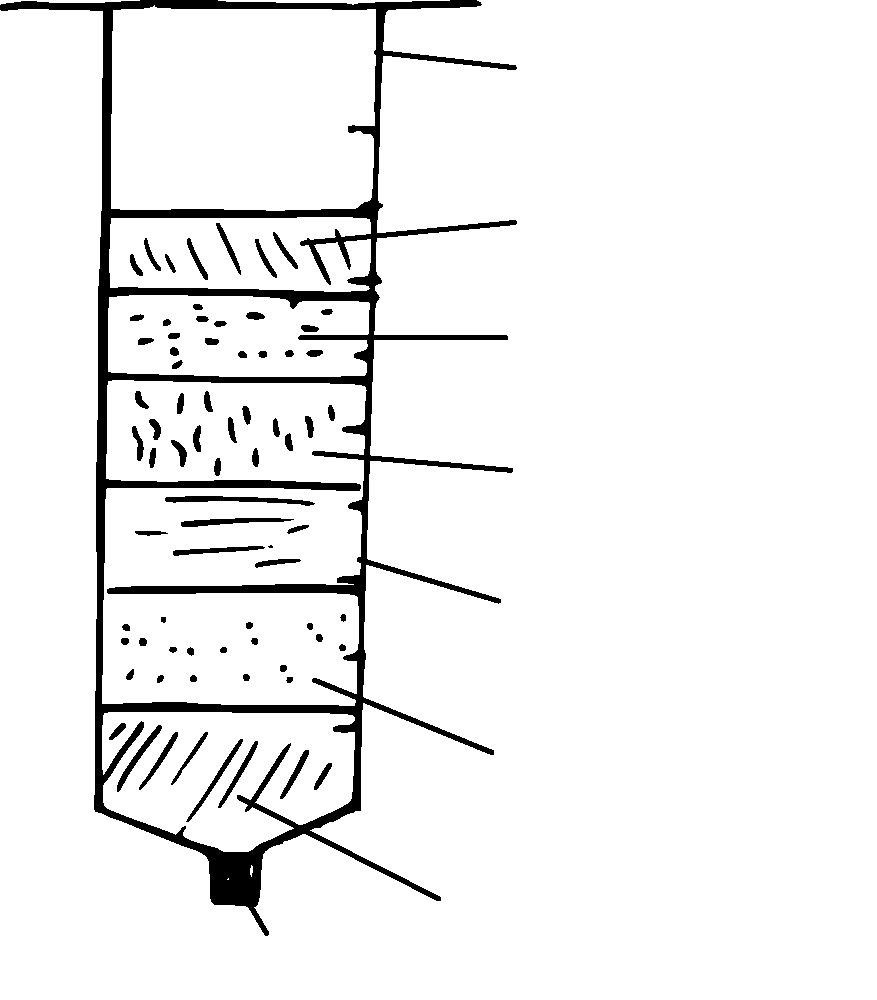
\includegraphics[width=0.3\textwidth]{./img/density-tower.png}
\end{center}

\begin{description*}
%\item[Subtopic:]{}
\item[Materials:]{Syringes, water, honey, glycerine, cooking oil, spirit, kerosene, erasers, paper clips, nails, other small objects}
%\item[Setup:]{}
\item[Procedure:]{Add each liquid into the syringe, one by one, observing the relative depths of each liquid. Place small solid objects e.g. rubber erasers, paper clips, small nails, etc. into the syringe and observe their positions relative to the various liquids.}
%\item[Hazards:]{}
\item[Questions:]{Which liquid is the most dense? Which is the least dense?}
\item[Observations:]{The denser liquids sink to the bottom while the less dense liquids rise to the top. The solid objects settle among liquids of comparable density.}
%\item[Theory:]{$ \mathrm{Density} = \mathrm{mass} \div \mathrm{Volume} $ ($ \rho = \cfrac{m}{V} $). Relative density (R.D.) can be used to compare the density of a given material to that of water. Liquids with a greater density sink to the bottom, while those having a lower density rise to the top.}
\item[Applications:]{Relative densities of liquids and solids help to identify certain substances, e.g. whether a ring is really made of gold.}
\item[Notes:]{Food coloring can be added to colorless liquids such as water, kerosene and glycerine to help distinguish among them.}
\end{description*}

%\subsection{Relative Density of a Liquid}

\subsection{U-Tube Apparatus}
\label{sub:u-tube}

\begin{description*}
%\item[Subtopic:]{}
\item[Materials:]{3 clear plastic pen tubes, cardboard, heated nail or knife, tape, pen, super glue, water, kerosene.}
\item[Setup:]{Cut two of the tubes at one end to make a 45$^\circ$ angle, and cut the third tube (shorter than the other two) to make a 45$^\circ$ angle at both ends. Attach the two longer tubes to either side of the short one so that they make right angles and form a U-shape. Melt the angled ends together with a hot knife, soldering iron, etc. so that the apparatus is water-tight. Glue the assembly to a cardboard base so that it stands upright. 

Place thin strips of tape along each side of the U-tube and mark with identical scales. Do this by adding known volumes of water and marking the levels on each scale. Label these marks from top to bottom as 0, 1, 2, etc.}
\item[Procedure:]{Place an amount of water into the U-tube such that the water rises about half way on either side of the tube. The actual volume of water is not important as long as you can see the levels clearly. Stand the tube upright and slowly drip about 1 mL of kerosene into one side of the U-tube. Measure the relative heights of water and the kerosene from the bottom level of the kerosene.}
%\item[Hazards:]{}
%\item[Questions:]{}
\item[Observations:]{The kerosene will displace the water, so you should see the water level on the other side rise slightly.}
\item[Theory:]{If a fluid’s density is less than that of water, it will float on top, displacing the water on the other side of the tube. From Archimedes’ principle and the Law of Flotation, we know that \[ \frac{\text{height of water}}{\text{height of kerosene}} = \frac{\text{density of kerosene}}{\text{density of water}} \]. The scales drawn on the outside of the U-tube allow us to find the ratio of the heights without needing units, and the density of water is known to be 1.0 g/mL, so the density of the other fluid can be calculated.}
%\item[Applications:]{}
\item[Notes:]{If the other fluid has a higher density than water, the experiment can still be done, but the fluid with higher density must be added first, then displaced with water, performing the same calculation.}
\end{description*}

\end{multicols}

\pagebreak